% uklad dokumentu
	\documentclass{article}
	\usepackage{xparse}
	\usepackage[margin=1cm]{geometry}
    \usepackage{enumerate} 
	\frenchspacing
    \linespread{1.2}
    \setlength{\parindent}{0pt}

% jezyk polski
	\usepackage[polish]{babel}
	\usepackage[utf8]{inputenc}
	\usepackage{polski}
 
% pakiety matematyczne
    \let\lll\undefined
	\usepackage{amssymb}
    \usepackage{amsthm}
	\usepackage{amsmath}
	\usepackage{amsfonts}
	\usepackage{tikz}

% hiperlacza
	\usepackage{hyperref}
	\hypersetup{
		colorlinks,
		citecolor=black,
		filecolor=black,
		linkcolor=black,
		urlcolor=black
	}

% wstawianie zdjec
	\usepackage{graphicx} 
	\pagenumbering{gobble}
	

% podstawowe informacje
    \title{Algorytmy metaheurystyczne 3}
    \author{Paweł Cegieła, Wojciech Sęk}

\begin{document} 

\maketitle

\section{Rodzaje algorytmu}
Rodzaje algorytmu - do zrobienia

\section{Parametry algorytmów}
Parametry algorytmów - do zrobienia

\section{Teoretyczna złożoność}
Teoretyczna złożoność - do zrobienia

\section{Wykonane eksperymenty}

Strojenie algorytmu zostało wykonane na podstawie danych z TSPLIB. Wybrane zostały parametry, dla których algorytm najlepiej zachowywał się podczas testowania. Jeśli jeden z dwóch parametrów miał np. lepsze wyniki od drugiego dla jednych danych (np. dla mniejszych wielkości macierzy), a gorsze dla innych, wybierany był jeden z tych parametrów po przemyśleniu.

Po strojeniu zostały przeprowadzone eksperymenty porównujące algorytm w wersji oraz z parametrami wybranymi jako domyślne: z innymi wersjami algorytmu oraz z tabu search, a także z różnymi wartościami parametrów. Nie w każdym eksperymencie czy nie dla każdego typu macierzy domyślny algorytm okazał się najlepszy, natomiast strojenie pomogło nam znaleźć taki algorytm oraz parametry, które średnio zachowują się najlepiej.

\subsection{Porównanie wersji algorytmu genetycznego i tabu search}

\begin{center}
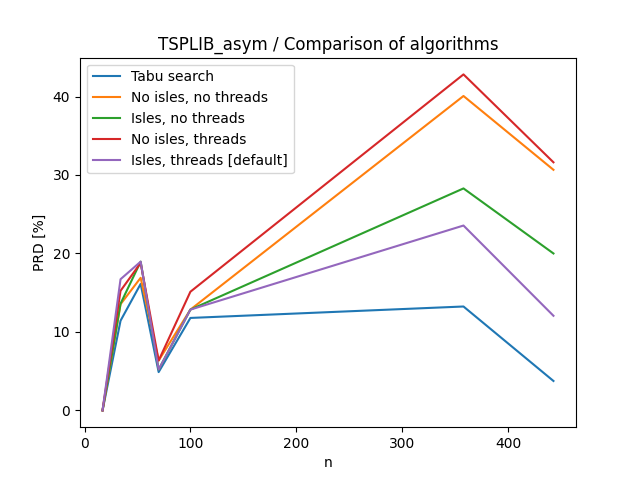
\includegraphics[width=\textwidth, 
                   height = 0.4\textheight, 
                   keepaspectratio]
                  {plots/tsplib_asym_1_comparison} 
\end{center}

\begin{center}
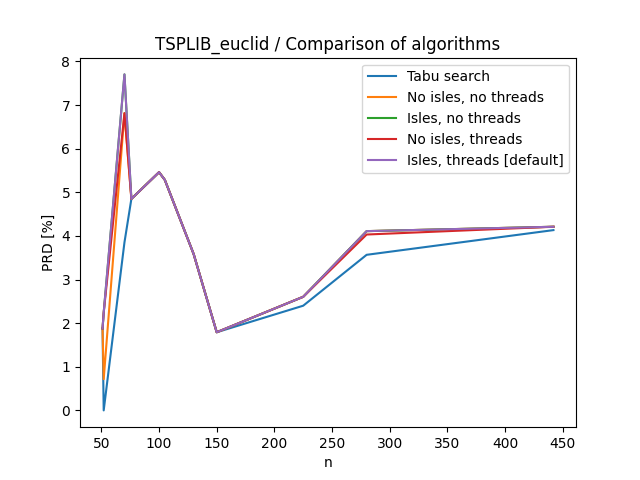
\includegraphics[width=\textwidth, 
                   height = 0.4\textheight, 
                   keepaspectratio]
                  {plots/tsplib_euclid_1_comparison} 
\end{center}

\begin{center}
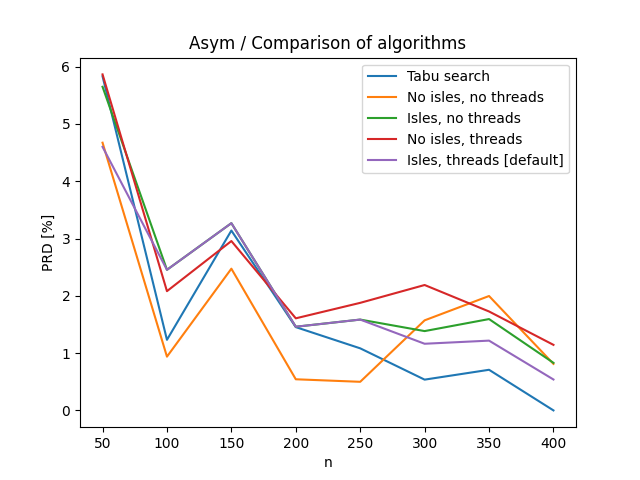
\includegraphics[width=\textwidth, 
                   height = 0.4\textheight, 
                   keepaspectratio]
                  {plots/asym_1_comparison} 
\end{center}

\begin{center}
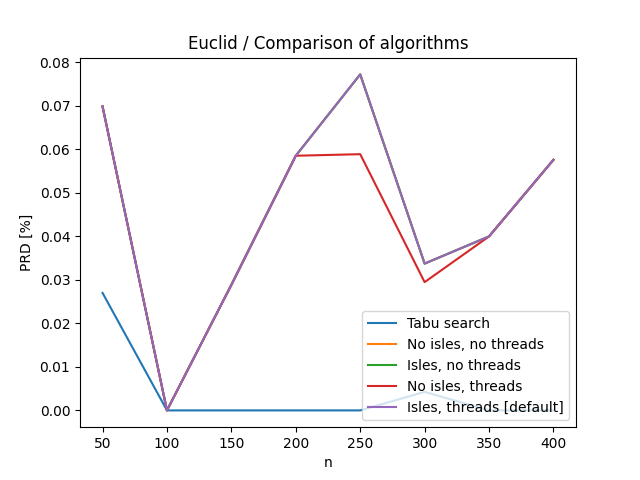
\includegraphics[width=\textwidth, 
                   height = 0.4\textheight, 
                   keepaspectratio]
                  {plots/euclid_1_comparison} 
\end{center}

\begin{center}
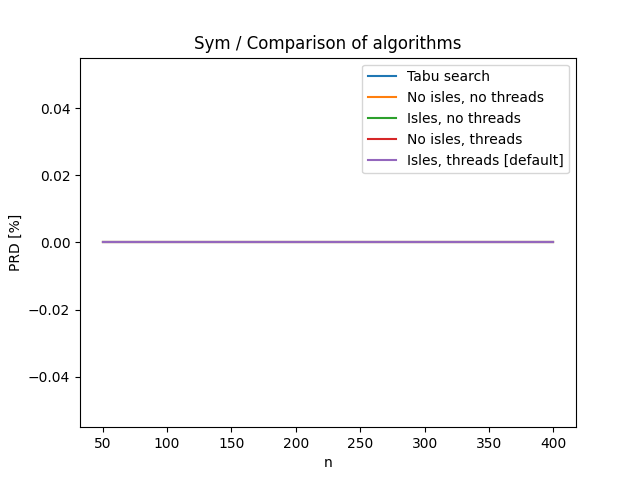
\includegraphics[width=\textwidth, 
                   height = 0.4\textheight, 
                   keepaspectratio]
                  {plots/sym_1_comparison} 
\end{center}


\subsection{Przybliżenie początkowe}

\begin{center}
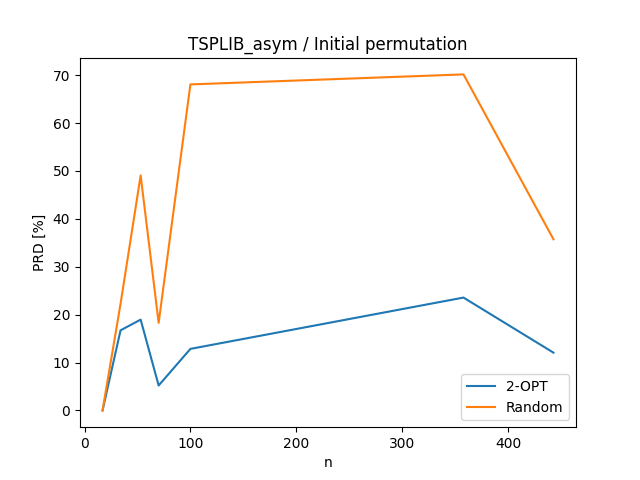
\includegraphics[width=\textwidth, 
                   height = 0.4\textheight, 
                   keepaspectratio]
                  {plots/tsplib_asym_2_gen_rand} 
\end{center}

\begin{center}
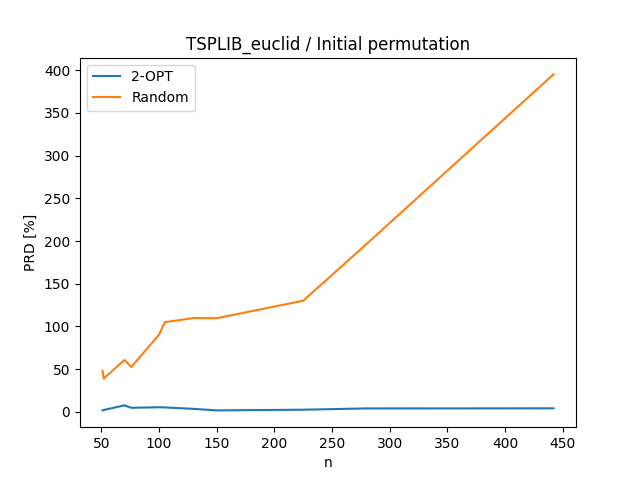
\includegraphics[width=\textwidth, 
                   height = 0.4\textheight, 
                   keepaspectratio]
                  {plots/tsplib_euclid_2_gen_rand} 
\end{center}

\begin{center}
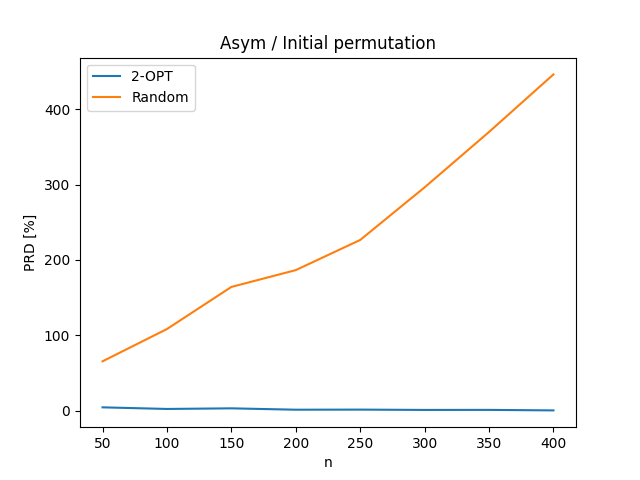
\includegraphics[width=\textwidth, 
                   height = 0.4\textheight, 
                   keepaspectratio]
                  {plots/asym_2_gen_rand} 
\end{center}

\begin{center}
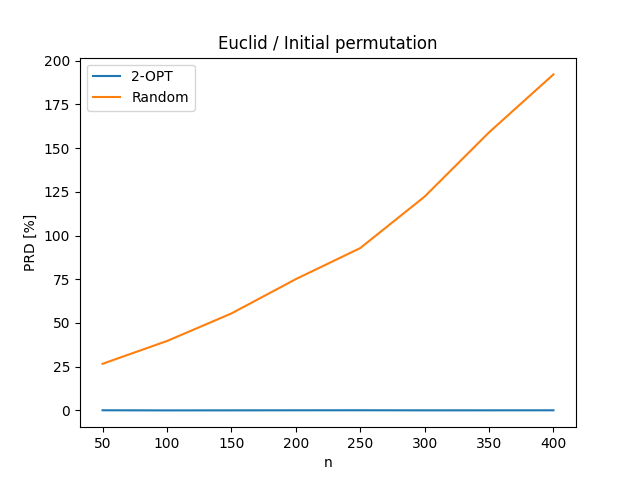
\includegraphics[width=\textwidth, 
                   height = 0.4\textheight, 
                   keepaspectratio]
                  {plots/euclid_2_gen_rand} 
\end{center}

\begin{center}
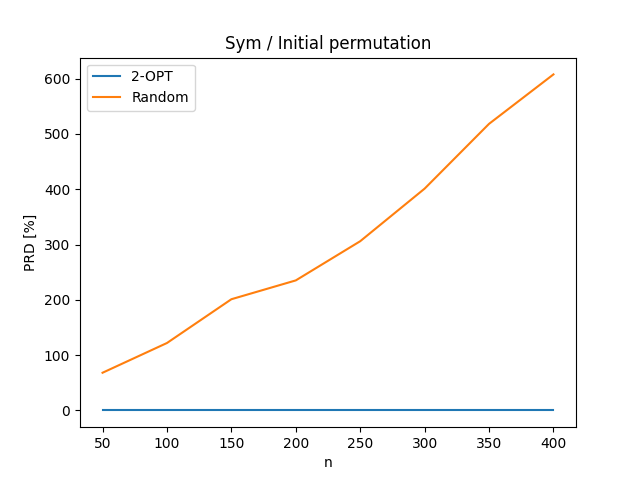
\includegraphics[width=\textwidth, 
                   height = 0.4\textheight, 
                   keepaspectratio]
                  {plots/sym_2_gen_rand} 
\end{center}


\subsection{Wielkość pokolenia}

\begin{center}
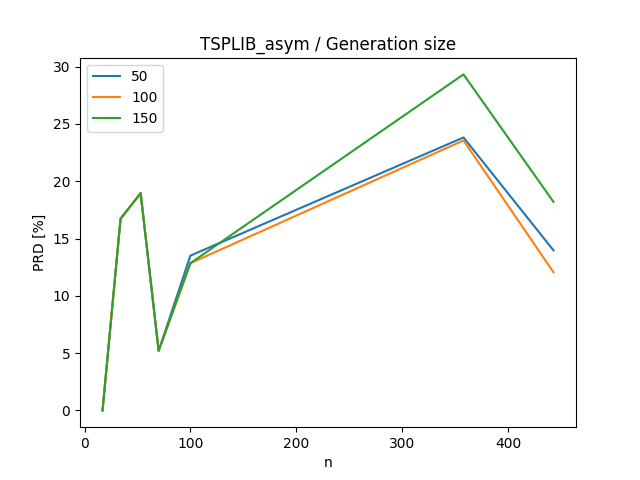
\includegraphics[width=\textwidth, 
                   height = 0.4\textheight, 
                   keepaspectratio]
                  {plots/tsplib_asym_3_generation_size} 
\end{center}

\begin{center}
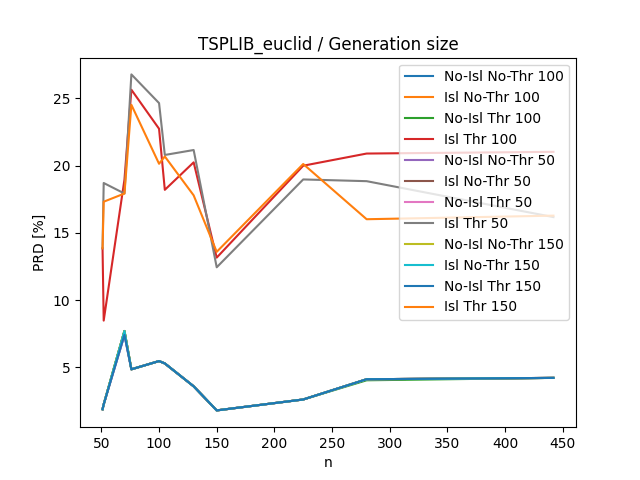
\includegraphics[width=\textwidth, 
                   height = 0.4\textheight, 
                   keepaspectratio]
                  {plots/tsplib_euclid_3_generation_size} 
\end{center}

\begin{center}
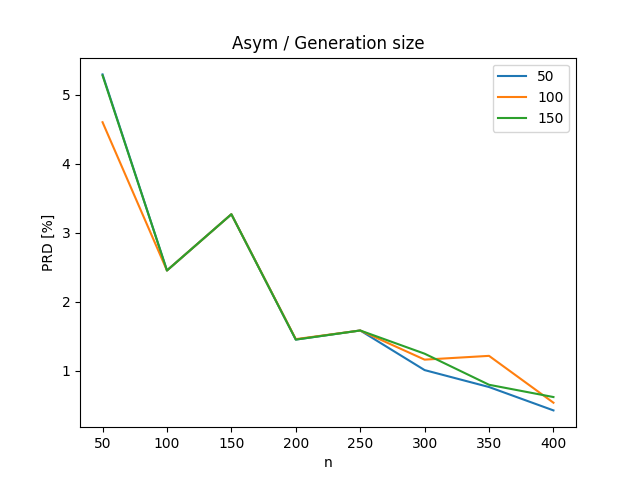
\includegraphics[width=\textwidth, 
                   height = 0.4\textheight, 
                   keepaspectratio]
                  {plots/asym_3_generation_size} 
\end{center}

\begin{center}
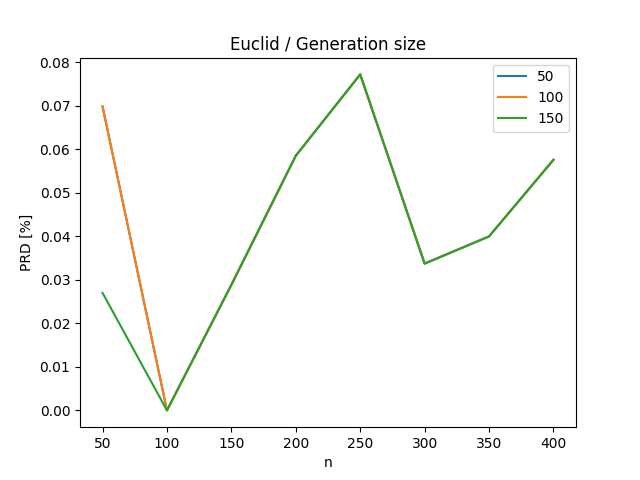
\includegraphics[width=\textwidth, 
                   height = 0.4\textheight, 
                   keepaspectratio]
                  {plots/euclid_3_generation_size} 
\end{center}

\begin{center}
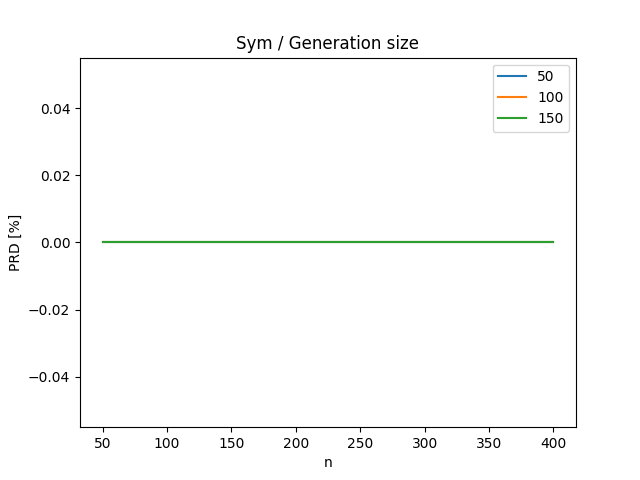
\includegraphics[width=\textwidth, 
                   height = 0.4\textheight, 
                   keepaspectratio]
                  {plots/sym_3_generation_size} 
\end{center}


\subsection{Wielkość elity}

\begin{center}
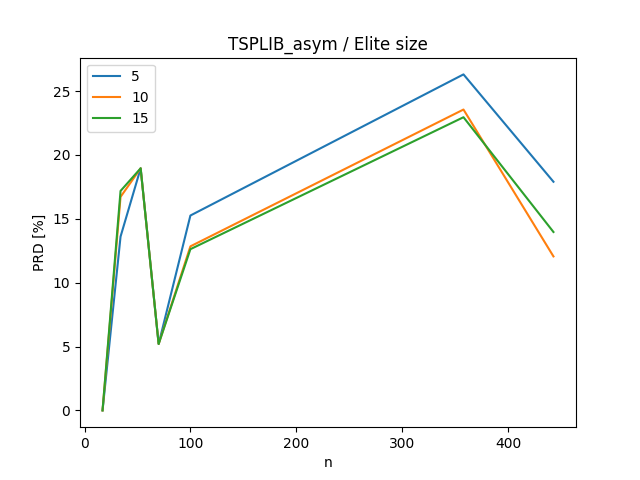
\includegraphics[width=\textwidth, 
                   height = 0.4\textheight, 
                   keepaspectratio]
                  {plots/tsplib_asym_4_elite_num} 
\end{center}

\begin{center}
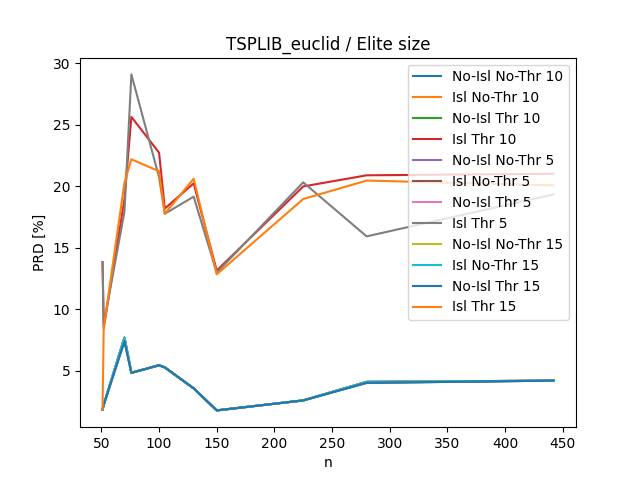
\includegraphics[width=\textwidth, 
                   height = 0.4\textheight, 
                   keepaspectratio]
                  {plots/tsplib_euclid_4_elite_num} 
\end{center}

\begin{center}
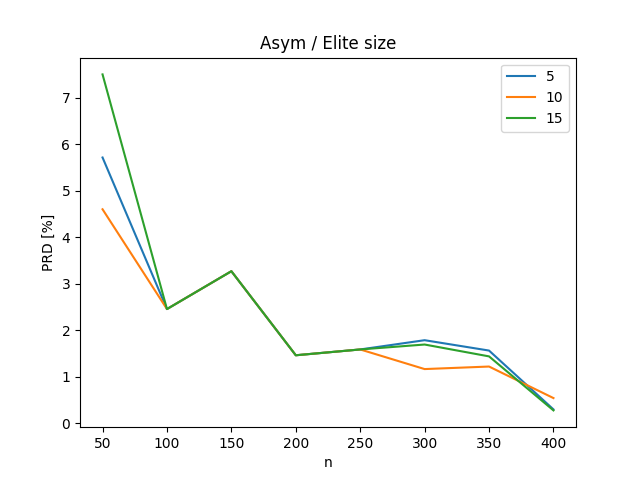
\includegraphics[width=\textwidth, 
                   height = 0.4\textheight, 
                   keepaspectratio]
                  {plots/asym_4_elite_num} 
\end{center}

\begin{center}
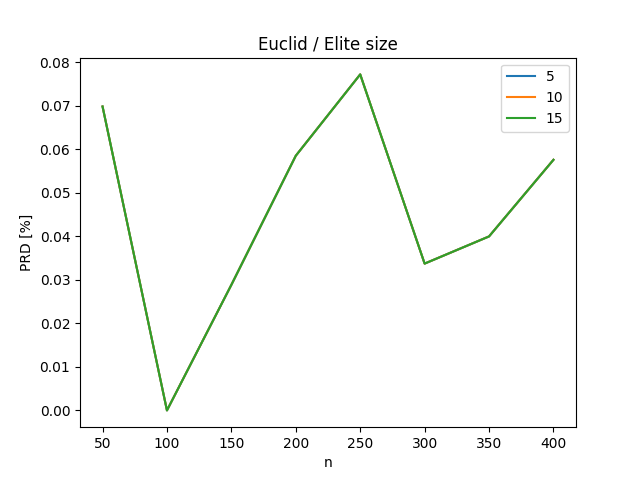
\includegraphics[width=\textwidth, 
                   height = 0.4\textheight, 
                   keepaspectratio]
                  {plots/euclid_4_elite_num} 
\end{center}

\begin{center}
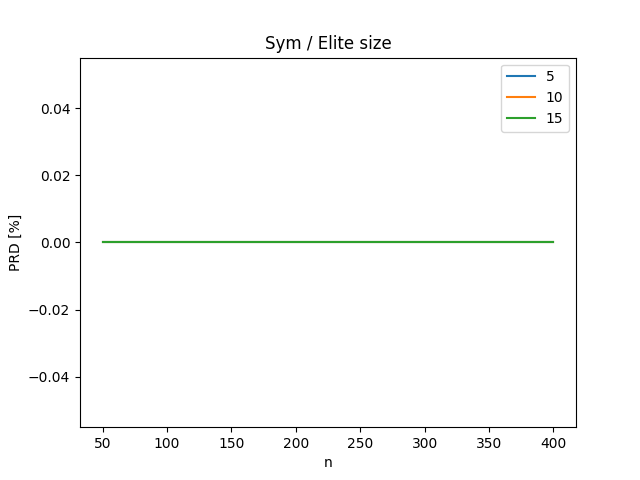
\includegraphics[width=\textwidth, 
                   height = 0.4\textheight, 
                   keepaspectratio]
                  {plots/sym_4_elite_num} 
\end{center}


\subsection{Krzyżowanie}

\begin{center}
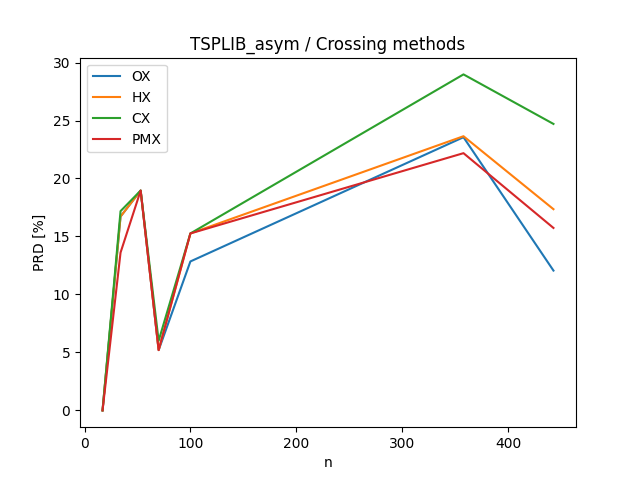
\includegraphics[width=\textwidth, 
                   height = 0.4\textheight, 
                   keepaspectratio]
                  {plots/tsplib_asym_5_crossing} 
\end{center}

\begin{center}
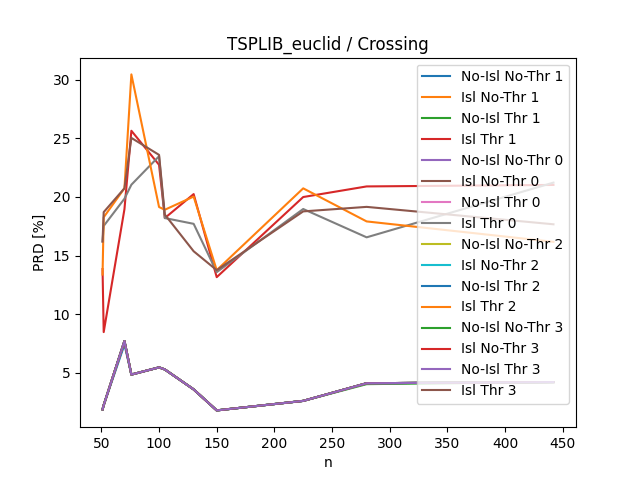
\includegraphics[width=\textwidth, 
                   height = 0.4\textheight, 
                   keepaspectratio]
                  {plots/tsplib_euclid_5_crossing} 
\end{center}

\begin{center}
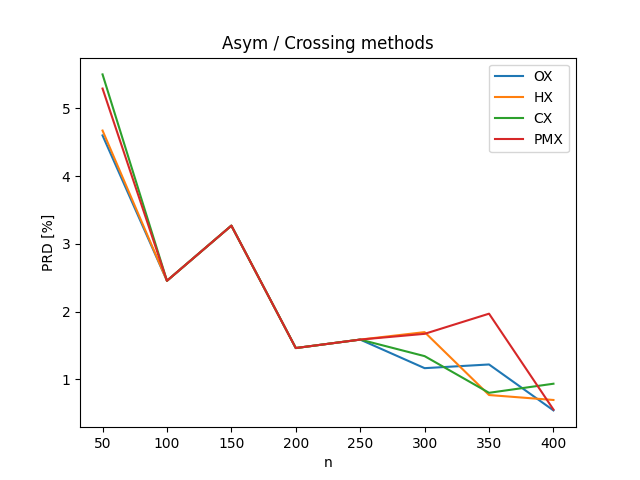
\includegraphics[width=\textwidth, 
                   height = 0.4\textheight, 
                   keepaspectratio]
                  {plots/asym_5_crossing} 
\end{center}

\begin{center}
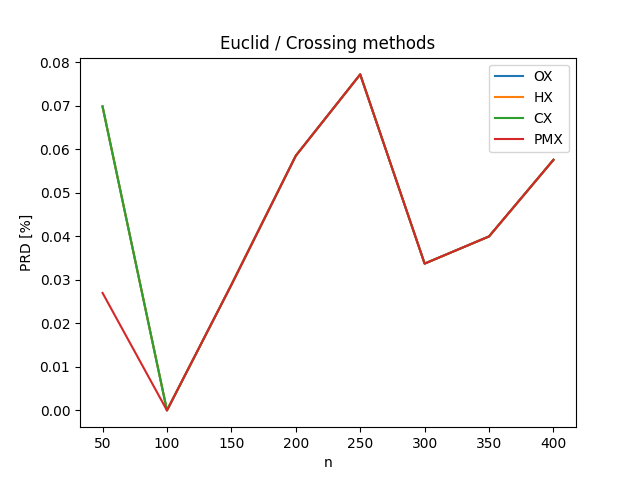
\includegraphics[width=\textwidth, 
                   height = 0.4\textheight, 
                   keepaspectratio]
                  {plots/euclid_5_crossing} 
\end{center}

\begin{center}
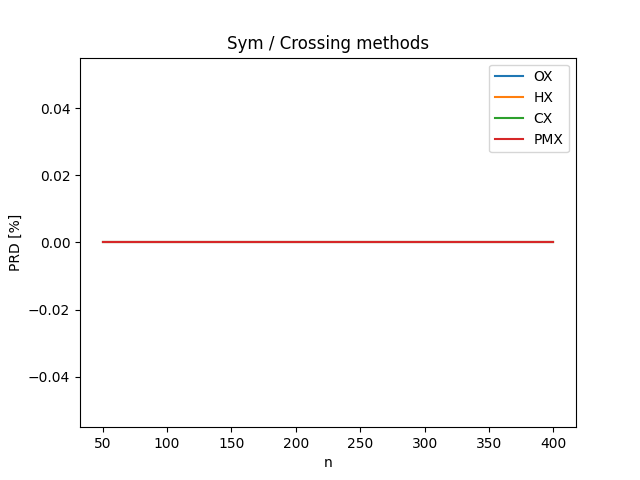
\includegraphics[width=\textwidth, 
                   height = 0.4\textheight, 
                   keepaspectratio]
                  {plots/sym_5_crossing} 
\end{center}


\subsection{Swap i inverse}

\begin{center}
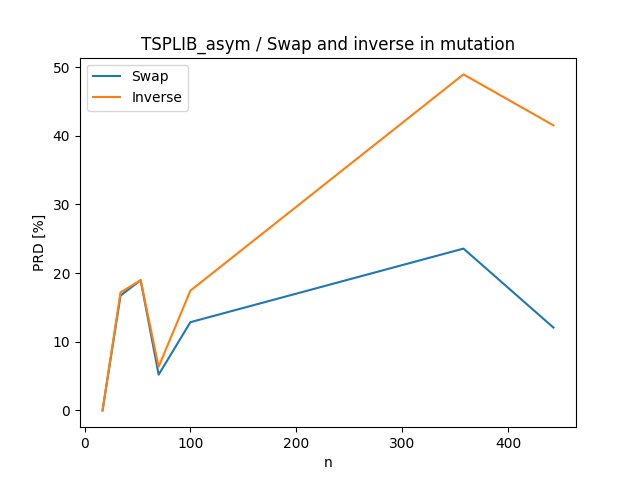
\includegraphics[width=\textwidth, 
                   height = 0.4\textheight, 
                   keepaspectratio]
                  {plots/tsplib_asym_6_swap_inverse} 
\end{center}

\begin{center}
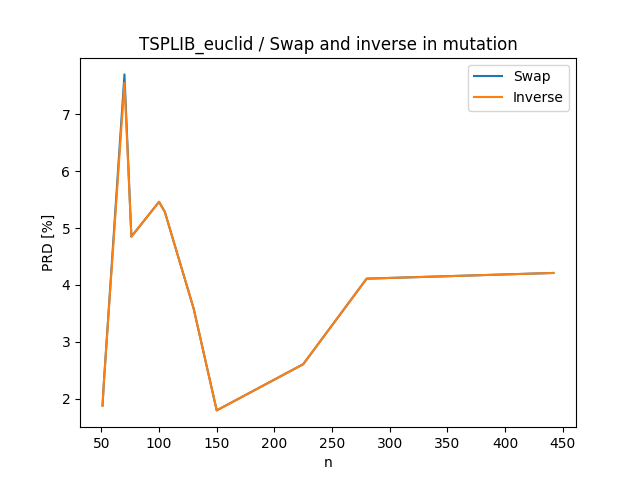
\includegraphics[width=\textwidth, 
                   height = 0.4\textheight, 
                   keepaspectratio]
                  {plots/tsplib_euclid_6_swap_inverse} 
\end{center}

\begin{center}
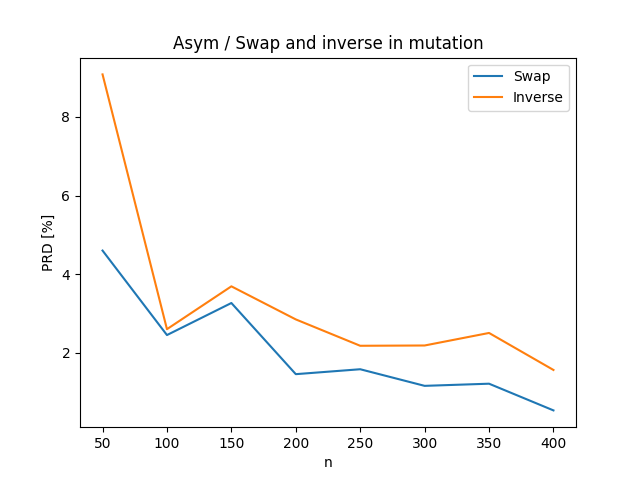
\includegraphics[width=\textwidth, 
                   height = 0.4\textheight, 
                   keepaspectratio]
                  {plots/asym_6_swap_inverse} 
\end{center}

\begin{center}
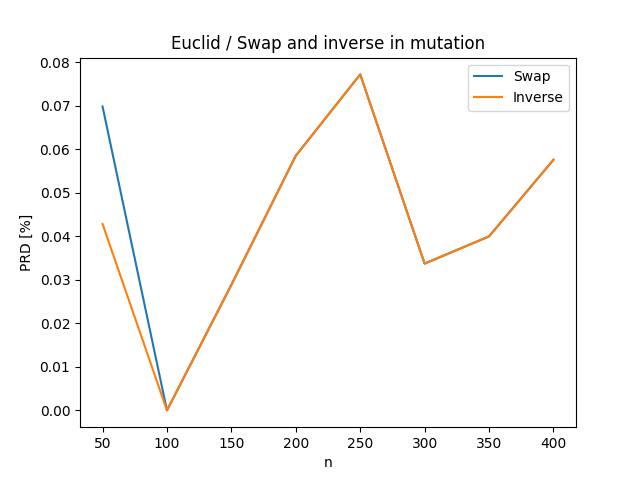
\includegraphics[width=\textwidth, 
                   height = 0.4\textheight, 
                   keepaspectratio]
                  {plots/euclid_6_swap_inverse} 
\end{center}

\begin{center}
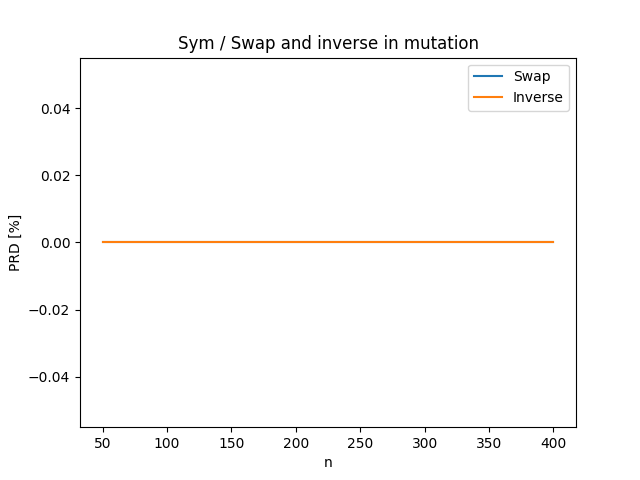
\includegraphics[width=\textwidth, 
                   height = 0.4\textheight, 
                   keepaspectratio]
                  {plots/sym_6_swap_inverse} 
\end{center}


\subsection{Turniej}

\begin{center}
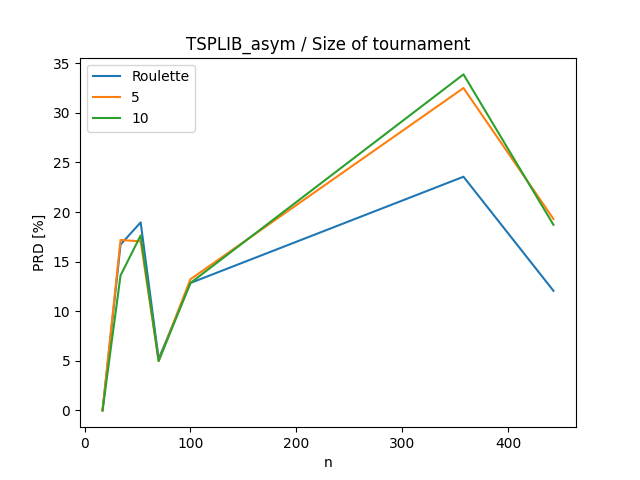
\includegraphics[width=\textwidth, 
                   height = 0.4\textheight, 
                   keepaspectratio]
                  {plots/tsplib_asym_7_tour} 
\end{center}

\begin{center}
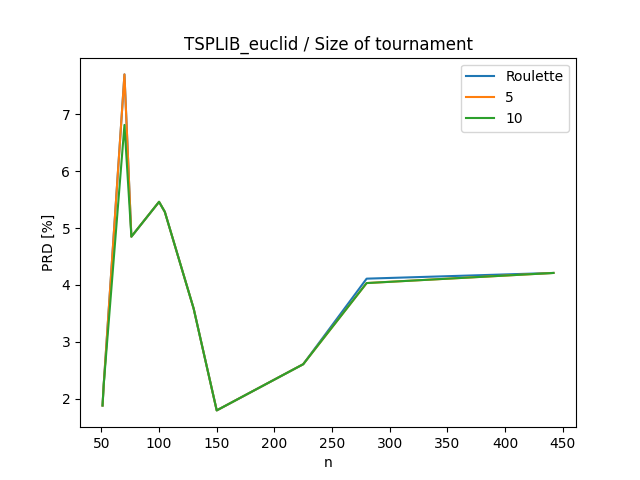
\includegraphics[width=\textwidth, 
                   height = 0.4\textheight, 
                   keepaspectratio]
                  {plots/tsplib_euclid_7_tour} 
\end{center}

\begin{center}
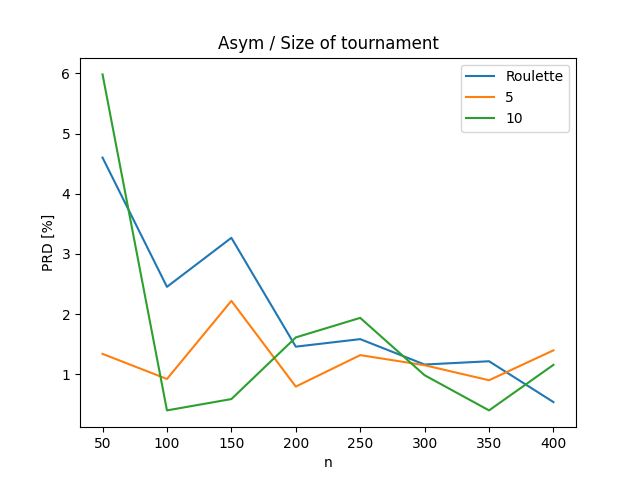
\includegraphics[width=\textwidth, 
                   height = 0.4\textheight, 
                   keepaspectratio]
                  {plots/asym_7_tour} 
\end{center}

\begin{center}
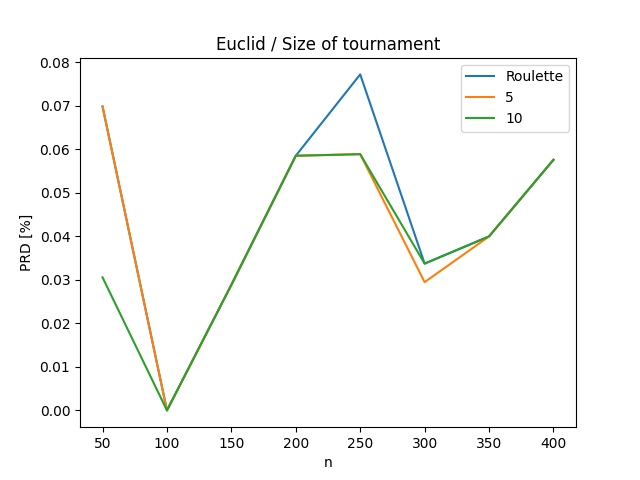
\includegraphics[width=\textwidth, 
                   height = 0.4\textheight, 
                   keepaspectratio]
                  {plots/euclid_7_tour} 
\end{center}

\begin{center}
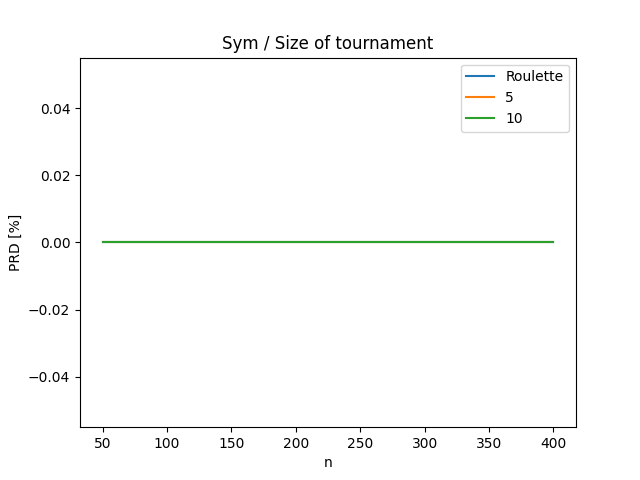
\includegraphics[width=\textwidth, 
                   height = 0.4\textheight, 
                   keepaspectratio]
                  {plots/sym_7_tour} 
\end{center}


\subsection{Szansa mutacji}

\begin{center}
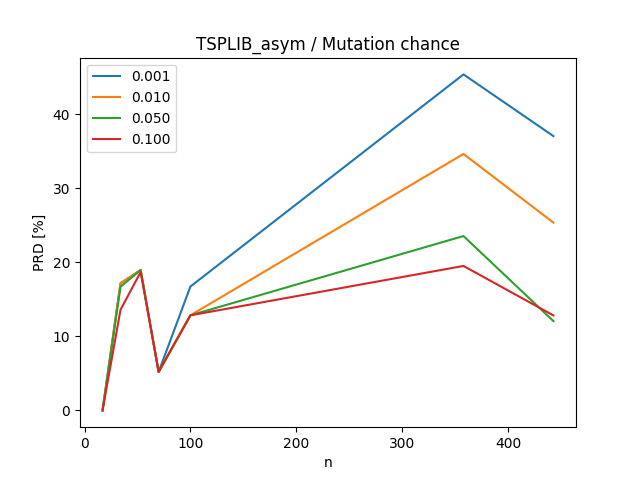
\includegraphics[width=\textwidth, 
                   height = 0.4\textheight, 
                   keepaspectratio]
                  {plots/tsplib_asym_8_mut_chance} 
\end{center}

\begin{center}
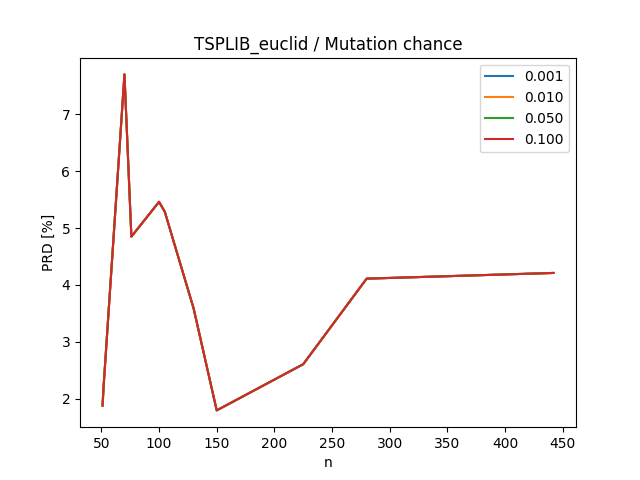
\includegraphics[width=\textwidth, 
                   height = 0.4\textheight, 
                   keepaspectratio]
                  {plots/tsplib_euclid_8_mut_chance} 
\end{center}

\begin{center}
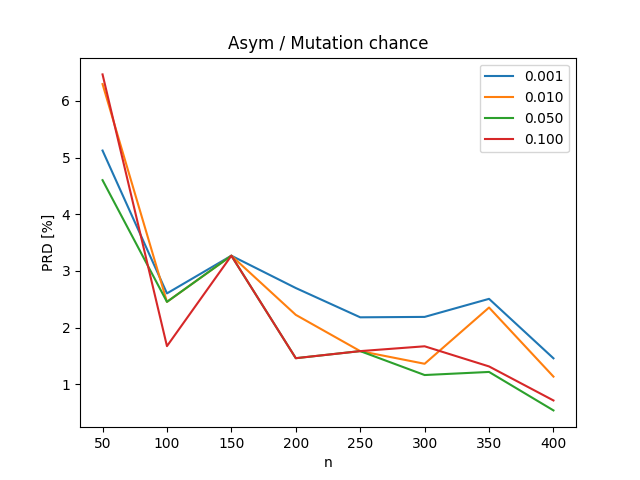
\includegraphics[width=\textwidth, 
                   height = 0.4\textheight, 
                   keepaspectratio]
                  {plots/asym_8_mut_chance} 
\end{center}

\begin{center}
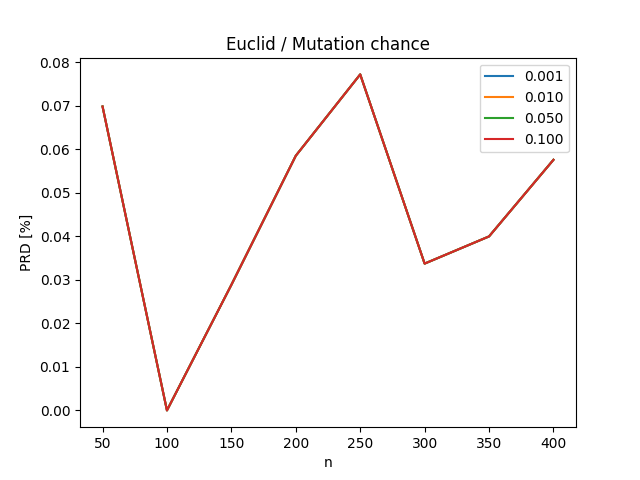
\includegraphics[width=\textwidth, 
                   height = 0.4\textheight, 
                   keepaspectratio]
                  {plots/euclid_8_mut_chance} 
\end{center}

\begin{center}
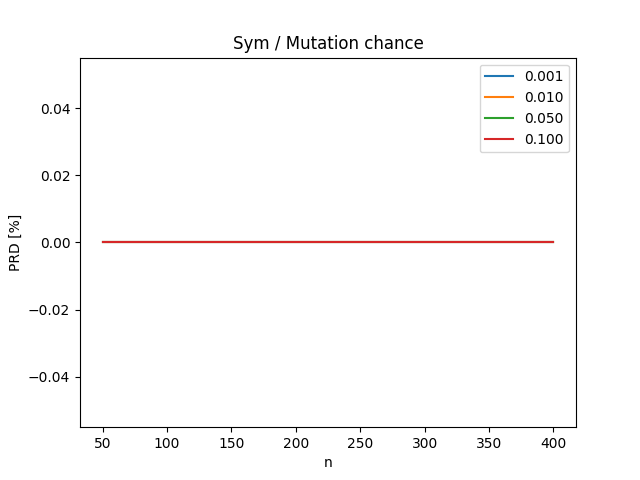
\includegraphics[width=\textwidth, 
                   height = 0.4\textheight, 
                   keepaspectratio]
                  {plots/sym_8_mut_chance} 
\end{center}


\subsection{Maksymalny czas}

\begin{center}
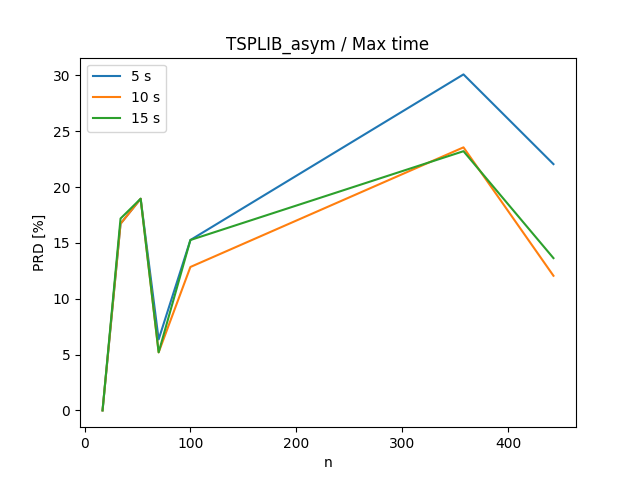
\includegraphics[width=\textwidth, 
                   height = 0.4\textheight, 
                   keepaspectratio]
                  {plots/tsplib_asym_9_max_time} 
\end{center}

\begin{center}
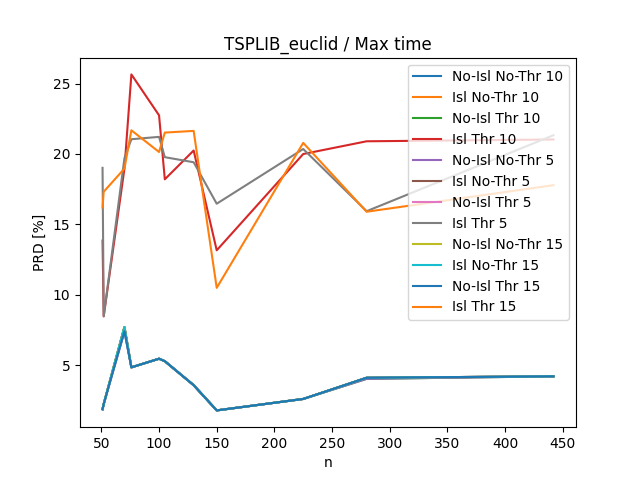
\includegraphics[width=\textwidth, 
                   height = 0.4\textheight, 
                   keepaspectratio]
                  {plots/tsplib_euclid_9_max_time} 
\end{center}

\begin{center}
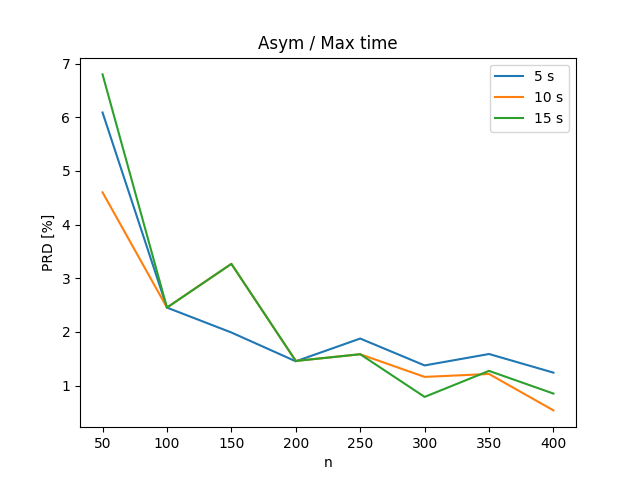
\includegraphics[width=\textwidth, 
                   height = 0.4\textheight, 
                   keepaspectratio]
                  {plots/asym_9_max_time} 
\end{center}

\begin{center}
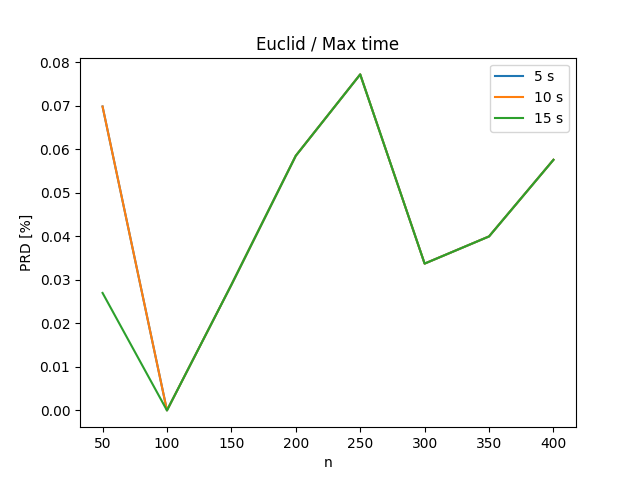
\includegraphics[width=\textwidth, 
                   height = 0.4\textheight, 
                   keepaspectratio]
                  {plots/euclid_9_max_time} 
\end{center}

\begin{center}
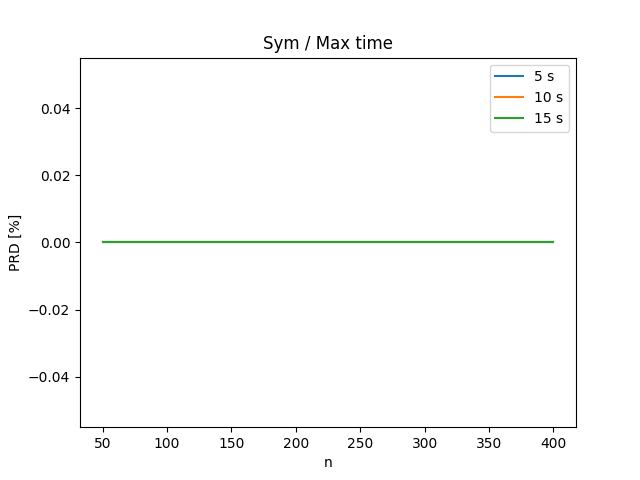
\includegraphics[width=\textwidth, 
                   height = 0.4\textheight, 
                   keepaspectratio]
                  {plots/sym_9_max_time} 
\end{center}


\subsection{Liczba wysp}

\begin{center}
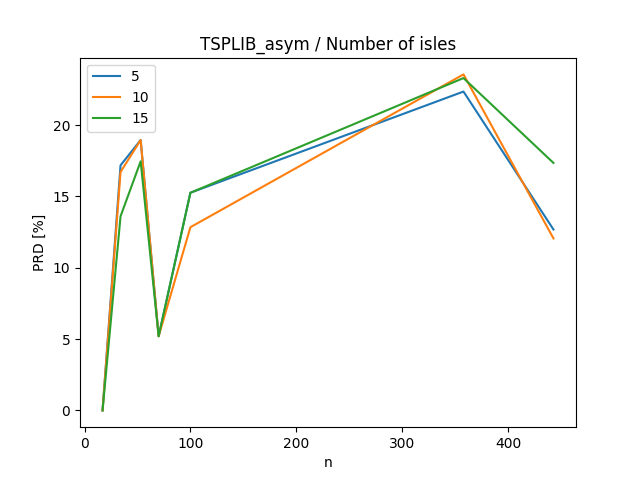
\includegraphics[width=\textwidth, 
                   height = 0.4\textheight, 
                   keepaspectratio]
                  {plots/tsplib_asym_10_isles} 
\end{center}

\begin{center}
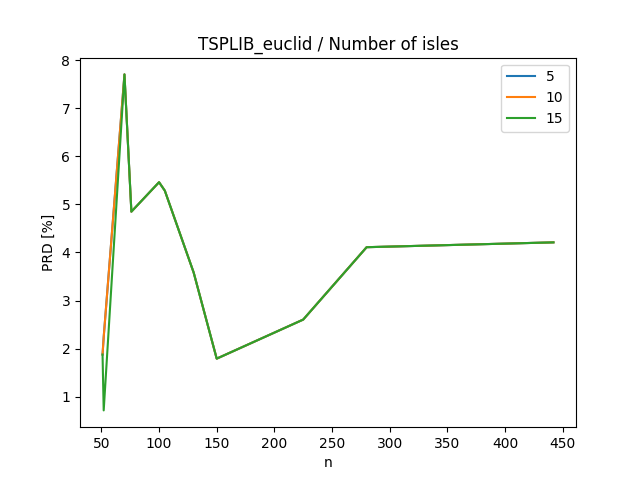
\includegraphics[width=\textwidth, 
                   height = 0.4\textheight, 
                   keepaspectratio]
                  {plots/tsplib_euclid_10_isles} 
\end{center}

\begin{center}
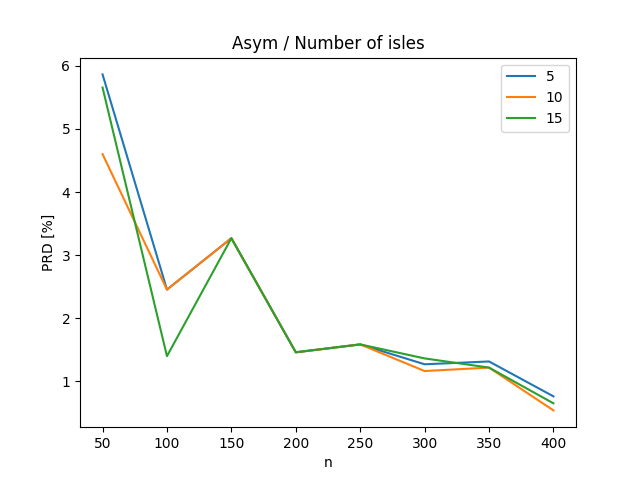
\includegraphics[width=\textwidth, 
                   height = 0.4\textheight, 
                   keepaspectratio]
                  {plots/asym_10_isles} 
\end{center}

\begin{center}
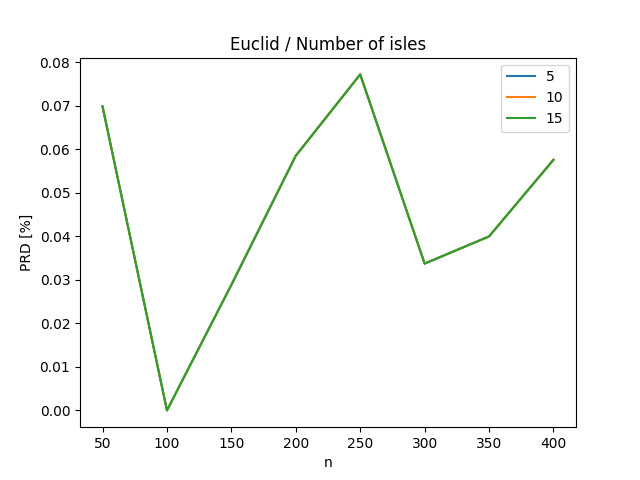
\includegraphics[width=\textwidth, 
                   height = 0.4\textheight, 
                   keepaspectratio]
                  {plots/euclid_10_isles} 
\end{center}

\begin{center}
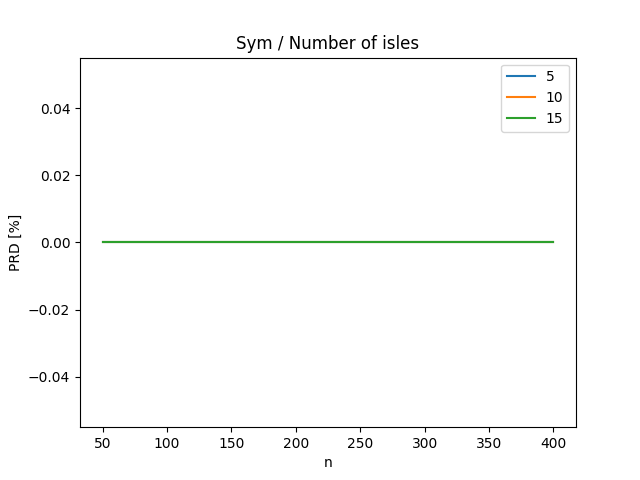
\includegraphics[width=\textwidth, 
                   height = 0.4\textheight, 
                   keepaspectratio]
                  {plots/sym_10_isles} 
\end{center}


\subsection{Częstotliwość migracji}

\begin{center}
\includegraphics[width=\textwidth, 
                   height = 0.4\textheight, 
                   keepaspectratio]
                  {plots/tsplib_asym_11_migration_freq} 
\end{center}

\begin{center}
\includegraphics[width=\textwidth, 
                   height = 0.4\textheight, 
                   keepaspectratio]
                  {plots/tsplib_euclid_11_migration_freq} 
\end{center}

\begin{center}
\includegraphics[width=\textwidth, 
                   height = 0.4\textheight, 
                   keepaspectratio]
                  {plots/asym_11_migration_freq} 
\end{center}

\begin{center}
\includegraphics[width=\textwidth, 
                   height = 0.4\textheight, 
                   keepaspectratio]
                  {plots/euclid_11_migration_freq} 
\end{center}

\begin{center}
\includegraphics[width=\textwidth, 
                   height = 0.4\textheight, 
                   keepaspectratio]
                  {plots/sym_11_migration_freq} 
\end{center}


\subsection{Liczba wątków}

\begin{center}
\includegraphics[width=\textwidth, 
                   height = 0.4\textheight, 
                   keepaspectratio]
                  {plots/tsplib_asym_12_num_of_threads} 
\end{center}

\begin{center}
\includegraphics[width=\textwidth, 
                   height = 0.4\textheight, 
                   keepaspectratio]
                  {plots/tsplib_euclid_12_num_of_threads} 
\end{center}

\begin{center}
\includegraphics[width=\textwidth, 
                   height = 0.4\textheight, 
                   keepaspectratio]
                  {plots/asym_12_num_of_threads} 
\end{center}

\begin{center}
\includegraphics[width=\textwidth, 
                   height = 0.4\textheight, 
                   keepaspectratio]
                  {plots/euclid_12_num_of_threads} 
\end{center}

\begin{center}
\includegraphics[width=\textwidth, 
                   height = 0.4\textheight, 
                   keepaspectratio]
                  {plots/sym_12_num_of_threads} 
\end{center}



\section{Obserwacje i wnioski}
\begin{itemize}
\item Obserwacje i wnioski - do zrobienia
\end{itemize}

\end{document}